% Options for packages loaded elsewhere
\PassOptionsToPackage{unicode}{hyperref}
\PassOptionsToPackage{hyphens}{url}
\PassOptionsToPackage{dvipsnames,svgnames,x11names}{xcolor}
%
\documentclass[
  letterpaper,
  DIV=11,
  numbers=noendperiod]{scrreprt}

\usepackage{amsmath,amssymb}
\usepackage{iftex}
\ifPDFTeX
  \usepackage[T1]{fontenc}
  \usepackage[utf8]{inputenc}
  \usepackage{textcomp} % provide euro and other symbols
\else % if luatex or xetex
  \usepackage{unicode-math}
  \defaultfontfeatures{Scale=MatchLowercase}
  \defaultfontfeatures[\rmfamily]{Ligatures=TeX,Scale=1}
\fi
\usepackage{lmodern}
\ifPDFTeX\else  
    % xetex/luatex font selection
\fi
% Use upquote if available, for straight quotes in verbatim environments
\IfFileExists{upquote.sty}{\usepackage{upquote}}{}
\IfFileExists{microtype.sty}{% use microtype if available
  \usepackage[]{microtype}
  \UseMicrotypeSet[protrusion]{basicmath} % disable protrusion for tt fonts
}{}
\makeatletter
\@ifundefined{KOMAClassName}{% if non-KOMA class
  \IfFileExists{parskip.sty}{%
    \usepackage{parskip}
  }{% else
    \setlength{\parindent}{0pt}
    \setlength{\parskip}{6pt plus 2pt minus 1pt}}
}{% if KOMA class
  \KOMAoptions{parskip=half}}
\makeatother
\usepackage{xcolor}
\setlength{\emergencystretch}{3em} % prevent overfull lines
\setcounter{secnumdepth}{5}
% Make \paragraph and \subparagraph free-standing
\makeatletter
\ifx\paragraph\undefined\else
  \let\oldparagraph\paragraph
  \renewcommand{\paragraph}{
    \@ifstar
      \xxxParagraphStar
      \xxxParagraphNoStar
  }
  \newcommand{\xxxParagraphStar}[1]{\oldparagraph*{#1}\mbox{}}
  \newcommand{\xxxParagraphNoStar}[1]{\oldparagraph{#1}\mbox{}}
\fi
\ifx\subparagraph\undefined\else
  \let\oldsubparagraph\subparagraph
  \renewcommand{\subparagraph}{
    \@ifstar
      \xxxSubParagraphStar
      \xxxSubParagraphNoStar
  }
  \newcommand{\xxxSubParagraphStar}[1]{\oldsubparagraph*{#1}\mbox{}}
  \newcommand{\xxxSubParagraphNoStar}[1]{\oldsubparagraph{#1}\mbox{}}
\fi
\makeatother


\providecommand{\tightlist}{%
  \setlength{\itemsep}{0pt}\setlength{\parskip}{0pt}}\usepackage{longtable,booktabs,array}
\usepackage{calc} % for calculating minipage widths
% Correct order of tables after \paragraph or \subparagraph
\usepackage{etoolbox}
\makeatletter
\patchcmd\longtable{\par}{\if@noskipsec\mbox{}\fi\par}{}{}
\makeatother
% Allow footnotes in longtable head/foot
\IfFileExists{footnotehyper.sty}{\usepackage{footnotehyper}}{\usepackage{footnote}}
\makesavenoteenv{longtable}
\usepackage{graphicx}
\makeatletter
\newsavebox\pandoc@box
\newcommand*\pandocbounded[1]{% scales image to fit in text height/width
  \sbox\pandoc@box{#1}%
  \Gscale@div\@tempa{\textheight}{\dimexpr\ht\pandoc@box+\dp\pandoc@box\relax}%
  \Gscale@div\@tempb{\linewidth}{\wd\pandoc@box}%
  \ifdim\@tempb\p@<\@tempa\p@\let\@tempa\@tempb\fi% select the smaller of both
  \ifdim\@tempa\p@<\p@\scalebox{\@tempa}{\usebox\pandoc@box}%
  \else\usebox{\pandoc@box}%
  \fi%
}
% Set default figure placement to htbp
\def\fps@figure{htbp}
\makeatother

\KOMAoption{captions}{tableheading}
\makeatletter
\@ifpackageloaded{tcolorbox}{}{\usepackage[skins,breakable]{tcolorbox}}
\@ifpackageloaded{fontawesome5}{}{\usepackage{fontawesome5}}
\definecolor{quarto-callout-color}{HTML}{909090}
\definecolor{quarto-callout-note-color}{HTML}{0758E5}
\definecolor{quarto-callout-important-color}{HTML}{CC1914}
\definecolor{quarto-callout-warning-color}{HTML}{EB9113}
\definecolor{quarto-callout-tip-color}{HTML}{00A047}
\definecolor{quarto-callout-caution-color}{HTML}{FC5300}
\definecolor{quarto-callout-color-frame}{HTML}{acacac}
\definecolor{quarto-callout-note-color-frame}{HTML}{4582ec}
\definecolor{quarto-callout-important-color-frame}{HTML}{d9534f}
\definecolor{quarto-callout-warning-color-frame}{HTML}{f0ad4e}
\definecolor{quarto-callout-tip-color-frame}{HTML}{02b875}
\definecolor{quarto-callout-caution-color-frame}{HTML}{fd7e14}
\makeatother
\makeatletter
\@ifpackageloaded{bookmark}{}{\usepackage{bookmark}}
\makeatother
\makeatletter
\@ifpackageloaded{caption}{}{\usepackage{caption}}
\AtBeginDocument{%
\ifdefined\contentsname
  \renewcommand*\contentsname{Table of contents}
\else
  \newcommand\contentsname{Table of contents}
\fi
\ifdefined\listfigurename
  \renewcommand*\listfigurename{List of Figures}
\else
  \newcommand\listfigurename{List of Figures}
\fi
\ifdefined\listtablename
  \renewcommand*\listtablename{List of Tables}
\else
  \newcommand\listtablename{List of Tables}
\fi
\ifdefined\figurename
  \renewcommand*\figurename{Figure}
\else
  \newcommand\figurename{Figure}
\fi
\ifdefined\tablename
  \renewcommand*\tablename{Table}
\else
  \newcommand\tablename{Table}
\fi
}
\@ifpackageloaded{float}{}{\usepackage{float}}
\floatstyle{ruled}
\@ifundefined{c@chapter}{\newfloat{codelisting}{h}{lop}}{\newfloat{codelisting}{h}{lop}[chapter]}
\floatname{codelisting}{Listing}
\newcommand*\listoflistings{\listof{codelisting}{List of Listings}}
\makeatother
\makeatletter
\makeatother
\makeatletter
\@ifpackageloaded{caption}{}{\usepackage{caption}}
\@ifpackageloaded{subcaption}{}{\usepackage{subcaption}}
\makeatother

\usepackage{bookmark}

\IfFileExists{xurl.sty}{\usepackage{xurl}}{} % add URL line breaks if available
\urlstyle{same} % disable monospaced font for URLs
\hypersetup{
  pdftitle={Exercise: Finding a Perpendicular Vector},
  pdfauthor={A},
  colorlinks=true,
  linkcolor={blue},
  filecolor={Maroon},
  citecolor={Blue},
  urlcolor={Blue},
  pdfcreator={LaTeX via pandoc}}


\title{Exercise: Finding a Perpendicular Vector}
\author{A}
\date{}

\begin{document}
\maketitle

\renewcommand*\contentsname{Table of contents}
{
\hypersetup{linkcolor=}
\setcounter{tocdepth}{2}
\tableofcontents
}

\bookmarksetup{startatroot}

\chapter{A}\label{a}

A

\begin{itemize}
\item
  https://www.youtube.com/watch?v=vNePhmCMnbU
\item
  https://www.youtube.com/watch?v=P3Y8OWkiUts
\end{itemize}

\part{Math \textbar{} Practical}

\chapter{Practice 1: Vectors}\label{practice-1-vectors}

\section{Exercise: Finding a Perpendicular
Vector}\label{exercise-finding-a-perpendicular-vector}

\textbf{Context:}\\
In linear algebra, two vectors are perpendicular (or orthogonal) if
their dot product is zero. In this exercise, you will find a vector in
\(\mathbb{R}^2\) that is perpendicular to a given vector.

\textbf{Given:}\\
Let \(\mathbf{v} = [2, 3]\).

\textbf{Tasks:}

\begin{enumerate}
\def\labelenumi{\arabic{enumi}.}
\tightlist
\item
  \textbf{Find a Perpendicular Vector:}

  \begin{itemize}
  \tightlist
  \item
    Find a non-zero vector \(\mathbf{w} = [x, y]\) such that
    \(\mathbf{v}\) and \(\mathbf{w}\) are perpendicular.
  \end{itemize}
\item
  \textbf{Verification:}

  \begin{itemize}
  \tightlist
  \item
    Show that your chosen vector \(\mathbf{w}\) indeed satisfies the
    condition \(\mathbf{v} \cdot \mathbf{w} = 0\).
  \end{itemize}
\item
  \textbf{Unit Perpendicular Vector:}

  \begin{itemize}
  \tightlist
  \item
    Find a unit vector in the direction of \(\mathbf{w}\) by computing
    \(\frac{\mathbf{w}}{\|\mathbf{w}\|}\), where \(\|\mathbf{w}\|\) is
    the Euclidean norm of \(\mathbf{w}\).
  \end{itemize}
\item
  \textbf{Bonus Discussion:}

  \begin{itemize}
  \tightlist
  \item
    Explain why there are infinitely many vectors perpendicular to
    \(\mathbf{v}\) and describe the general form of all such vectors.
  \end{itemize}
\end{enumerate}

\begin{center}\rule{0.5\linewidth}{0.5pt}\end{center}

\section{Exercise: Finding the Closest Word with 2D
Embeddings}\label{exercise-finding-the-closest-word-with-2d-embeddings}

\textbf{Context:}\\
In NLP, words can be represented as vectors. Here, each word is
represented by a 2-dimensional vector. By comparing these vectors using
Euclidean distance and cosine similarity, you can determine which word
is ``closer'' in meaning.

\textbf{Given Word Embeddings:}

\begin{itemize}
\tightlist
\item
  \textbf{cheese:} \texttt{{[}1,\ 2{]}}
\item
  \textbf{mushroom:} \texttt{{[}3,\ 1{]}}
\item
  \textbf{tasty:} \texttt{{[}2,\ 2{]}}
\end{itemize}

\textbf{Tasks:}

\begin{enumerate}
\def\labelenumi{\arabic{enumi}.}
\tightlist
\item
  \textbf{Euclidean Distance:}

  \begin{itemize}
  \tightlist
  \item
    \textbf{a.} Compute the Euclidean distance between \textbf{tasty}
    and \textbf{cheese}.\\
  \item
    \textbf{b.} Compute the Euclidean distance between \textbf{tasty}
    and \textbf{mushroom}.\\
  \item
    \textbf{c.} Which word is closer to \textbf{tasty} based on the
    Euclidean distance?
  \end{itemize}
\item
  \textbf{Cosine Similarity:}\\
  \[
   \cos(\theta)=\frac{\mathbf{u}\cdot\mathbf{v}}{\|\mathbf{u}\|\|\mathbf{v}\|}
  \]

  \begin{itemize}
  \tightlist
  \item
    \textbf{a.} Compute the cosine similarity between \textbf{tasty} and
    \textbf{cheese} using the formula above.
  \item
    \textbf{b.} Compute the cosine similarity between \textbf{tasty} and
    \textbf{mushroom}.\\
  \item
    \textbf{c.} Based on cosine similarity, which word is closer to
    \textbf{tasty}?
  \end{itemize}
\item
  \textbf{Discussion:}

  \begin{itemize}
  \tightlist
  \item
    Compare the outcomes from the Euclidean distance and cosine
    similarity calculations.\\
  \item
    Discuss why one metric might be preferred over the other in
    different NLP applications.
  \end{itemize}
\end{enumerate}

\begin{tcolorbox}[enhanced jigsaw, toptitle=1mm, titlerule=0mm, toprule=.15mm, bottomtitle=1mm, opacityback=0, opacitybacktitle=0.6, bottomrule=.15mm, title=\textcolor{quarto-callout-note-color}{\faInfo}\hspace{0.5em}{Note}, leftrule=.75mm, arc=.35mm, colbacktitle=quarto-callout-note-color!10!white, rightrule=.15mm, left=2mm, colback=white, colframe=quarto-callout-note-color-frame, breakable, coltitle=black]

Cool video by 3blue1brown discussing
\href{https://youtu.be/wjZofJX0v4M?t=751}{word vectors (embeddings)}

\end{tcolorbox}

\section{Exercise: Linear transformation matrix
power}\label{exercise-linear-transformation-matrix-power}

\textbf{Tasks:} 1. \textbf{Matrix Power:}\\
- Compute the matrix power of the following matrix \(A\) to the power of
\(n\): \[
A = \begin{pmatrix}
    2 & 0 \\
    0 & -1
\end{pmatrix}
\] - What does the result represent in terms of linear transformations?

\section{Exercise: Subspace}\label{exercise-subspace}

\textbf{Tasks:}

Հարթության կոոդինատական համակարգի սկզբնակետից ելնող վեկտորների հետևյալ
բազմություններից յուրաքանչյուրի համար պարզել արդյոք այն գծային
ենթատարածություն է. \n

բոլոր վեկտորները որոնց վերջնակետերը ընկած են տրված ուղղի վրա

բոլոր վեկտորները որոնց վերջնակետերը ընկած չեն տրված ուղղի վրա

բոլոր վեկտորները որոնց վերջնակետերը ընկած են կոորդինատական համակարգի
առաջին քառորդում

բոլոր վեկտորները որոնց վերջնակետերը ընկած են կոորդինատական համակարգի
առաջին կամ երրորդ քառորդում

\section{Exercise: Vector Space}\label{exercise-vector-space}

\begin{figure}[H]

{\centering \pandocbounded{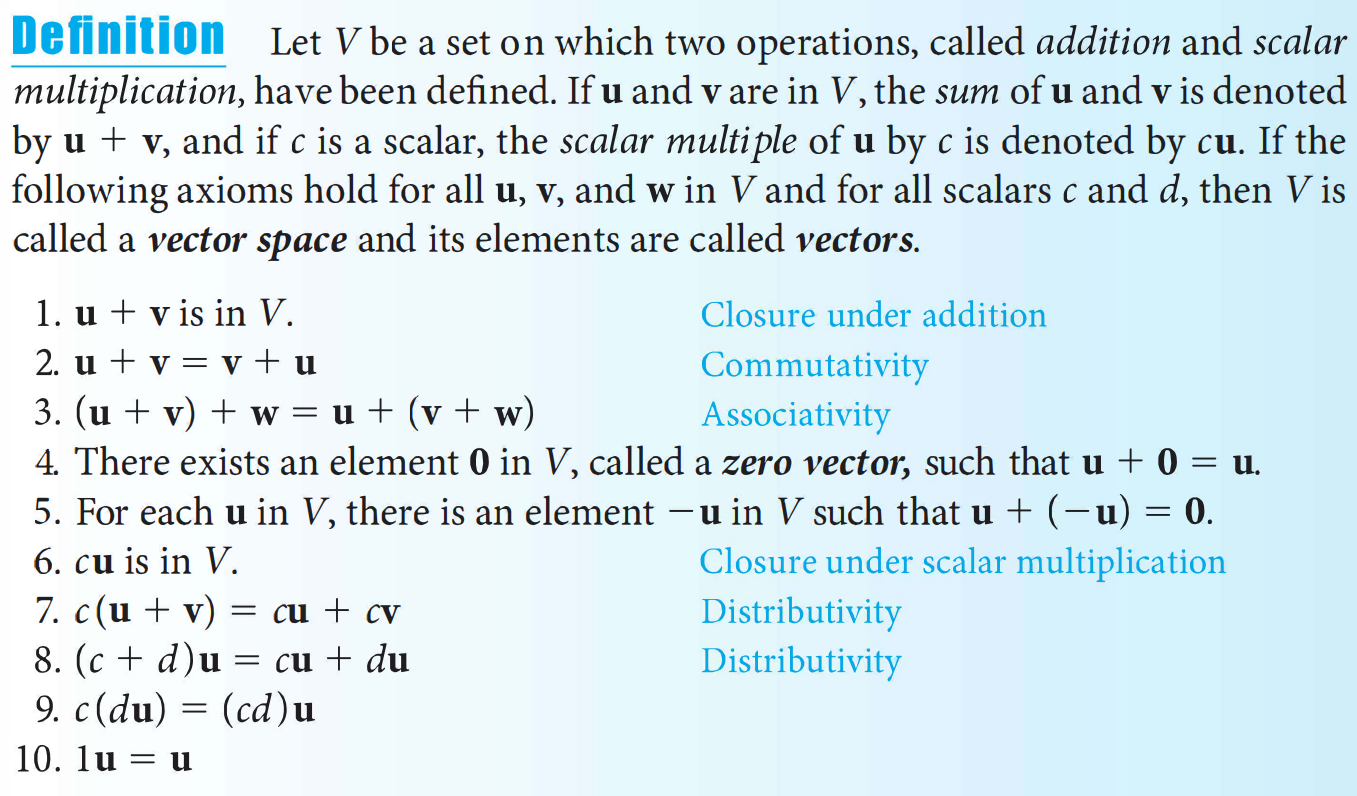
\includegraphics[keepaspectratio]{math/Resources/pr/vector_space.png}}

}

\caption{Poole\_vec\_space}

\end{figure}%




\end{document}
